%! TeX program = lualatex
\documentclass[a4paper]{article} 

% packages
\usepackage{microtype}      % Slightly tweak font spacing for aesthetics
\usepackage[english]{babel} % Language hyphenation and typographical rules
\usepackage{changepage}     % adjust margins on the fly

\usepackage[final, colorlinks = true, urlcolor = black, linkcolor = black, citecolor = black]{hyperref} 
\usepackage{fontspec}
% \setmainfont{EB Garamond}
% \setmonofont[Scale=MatchLowercase]{Deja Vu Sans Mono}

\setmainfont{EB Garamond}[
    Ligatures=TeX,
    Numbers=OldStyle
]

% Fallback font (for missing characters)
\setmainfont{EB Garamond}[
    % Ligatures=TeX,
    % Numbers=OldStyle
]

\newfontfamily{\emojifont}{Noto Color Emoji}[Renderer=Harfbuzz]

% Monospace font configuration
\setmonofont[Scale=MatchLowercase]{DejaVu Sans Mono}

\usepackage[backend=biber, style=numeric, date=iso, urldate=iso]{biblatex}
\addbibresource{references.bib}
\DeclareFieldFormat{urldate}{Accessed on: #1}

\usepackage{minted}
\usemintedstyle{algol_nu}
\usepackage{xcolor}

\usepackage{pgfplots}
\pgfplotsset{width=\textwidth,compat=1.9}

\usepackage{caption}
\newenvironment{code}{\captionsetup{type=listing}}{}
\captionsetup[listing]{skip=0pt}
\setlength{\abovecaptionskip}{5pt}
\setlength{\belowcaptionskip}{5pt}

\usepackage[yyyymmdd]{datetime}
\renewcommand{\dateseparator}{--}

\usepackage{titlesec}
% \titleformat{\section}{\LARGE\bfseries}{}{}{}[\titlerule]
% \titleformat{\subsection}{\Large\bfseries}{}{0em}{}
% \titlespacing{\subsection}{0em}{-0.7em}{0em}
%
% \titleformat{\subsubsection}{\large\bfseries}{}{0em}{$\bullet$ }
% \titlespacing{\subsubsection}{1em}{-0.7em}{0em}

% margins
\addtolength{\hoffset}{-2.25cm}
\addtolength{\textwidth}{4.5cm}
\addtolength{\voffset}{-3.25cm}
\addtolength{\textheight}{5cm}
\setlength{\parskip}{0pt}
\setlength{\parindent}{0in}
% \setcounter{secnumdepth}{0}

\begin{document}
\hrule \medskip
\begin{minipage}{0.295\textwidth} 
    \raggedright
    \footnotesize 
    \begin{tabular}{@{}l l}
        Name: & Andrew Hayes \\
        Student ID: & 21321503 \\
        E-mail: & \href{mailto://a.hayes18@universityofgalway.ie}{\texttt{a.hayes18@universityofgalway.ie}} \\
    \end{tabular}
\end{minipage}
\begin{minipage}{0.4\textwidth} 
    \centering 
    \vspace{0.4em}
    \LARGE
    \textsc{ct420} \\ 
\end{minipage}
\begin{minipage}{0.295\textwidth} 
    \raggedleft
    \today
\end{minipage}
\medskip\hrule 
\begin{center}
    \normalsize
    Assignment 2: POSIX Programming \& Benchmarking
\end{center}
\hrule
\medskip

\section{Host Environment}
For my host environment, I chose to run Ubuntu Server 24.04.2 LTS using a VirtualBox hypervisor.
I chose this operating system as I have sufficient Linux experience to feel confident using an operating system with no graphical interface (as opposed to Ubuntu Desktop), and the absence of a GUI means a smaller ISO file, memory footprint, \& CPU footprint.
I chose Ubuntu specifically because it's a Linux system with which I have previous experience, and is well-document with plenty of packages available to install if needs be.
Ubuntu also makes it easy to install the \verb|PREEMPT_RT| patches, which transform the standard Linux kernel into a fully preemptible, real-time kernel, which I felt was more suitable for this assignment, as the standard Linux kernel is not suitable for a hard real-time system due to its lack of preemption.

\begin{figure}[H]
    \centering
    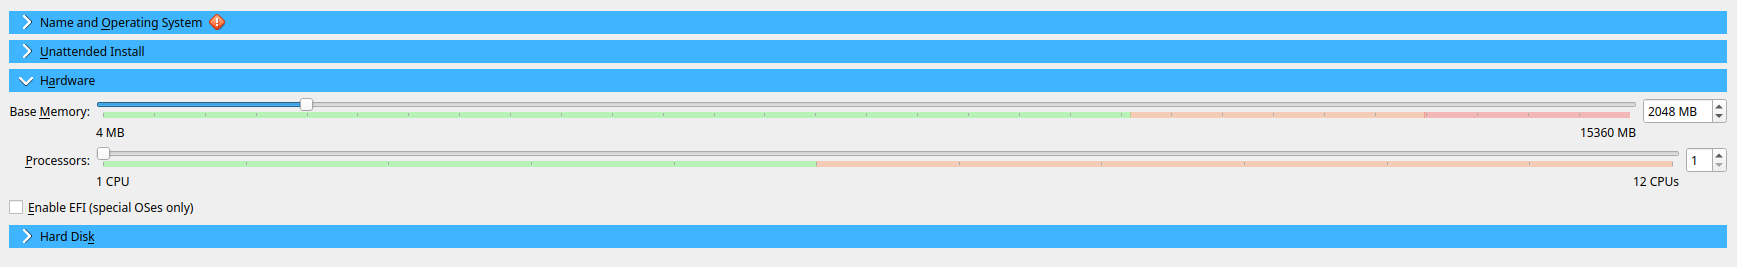
\includegraphics[width=\textwidth]{./images/hardware.png}
    \caption{Virtual machine hardware configuration}
\end{figure}

I set the virtual machine to have a single CPU and set the amount of RAM to 2048MB which is the recommended minimum for Ubuntu Server\supercite{ubuntu_server_installation}.
I left the hard disk size at the default of 25GB as I saw no reason to change it.
The real-time kernel with the \verb|PREEMPT_RT| patches installed is available with Ubuntu Pro, which is free for personal use.
After setting up an Ubuntu Pro account, I enabled the real-time kernel using the \mintinline{bash}{pro} command.

\begin{figure}[H]
    \centering
    
\includegraphics[width=\textwidth]{./images/proenable.png}
    \caption{Enabling the real-time kernel with the \mintinline{bash}{pro} command}
\end{figure}

Finally, I transferred over the following C file (taken from the lecture slides) via \mintinline{shell}{scp} to the virtual machine to get the clock resolution, which is 1 nanosecond:
\begin{code}
\begin{minted}[linenos, breaklines, frame=single]{C}
#include<unistd.h>
#include<time.h>
#include <stdio.h>

int main(){
    struct timespec clock_res;
    int stat;
    stat=clock_getres(CLOCK_REALTIME, &clock_res);
    printf("Clock resolution is %d seconds, %ld nanoseconds\n",clock_res.tv_sec,clock_res.tv_nsec);
    return 0;
}
\end{minted}
\end{code}

\begin{figure}[H]
    \centering
    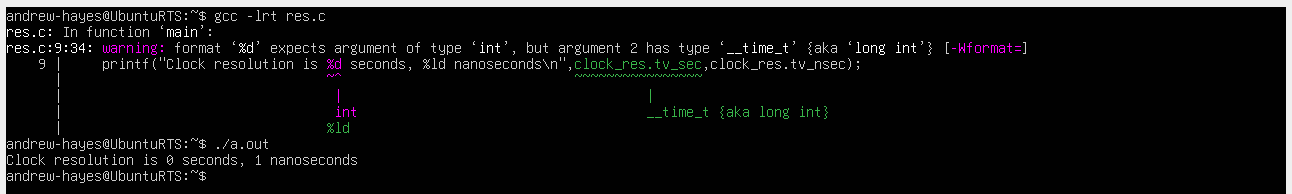
\includegraphics[width=\textwidth]{./images/clockres.png}
    \caption{Getting the clock resolution of the virtual machine}
\end{figure}

\section{CPU \& Data-Intensive Applications}
To develop my CPU \& data-intensive programs, I chose to use Python for ease of development (and because any Python program will stress your CPU \& memory no matter how simple {\emojifont 😉}).
I chose \mintinline{shell}{htop} as my resource-monitoring tool as I have often used it in the past, it has easy to read \& understand output, and shows you exactly what proportion of the CPU \& memory is in use at that time.
It also allows you to list processes by CPU consumption or memory consumption which is a useful option to have for this assignment.

\begin{code}
\inputminted[linenos, breaklines, frame=single]{python}{../code/stressers/stress_cpu.py}
\caption{\texttt{stress\_cpu.py}}
\end{code}

\begin{figure}[H]
    \centering
    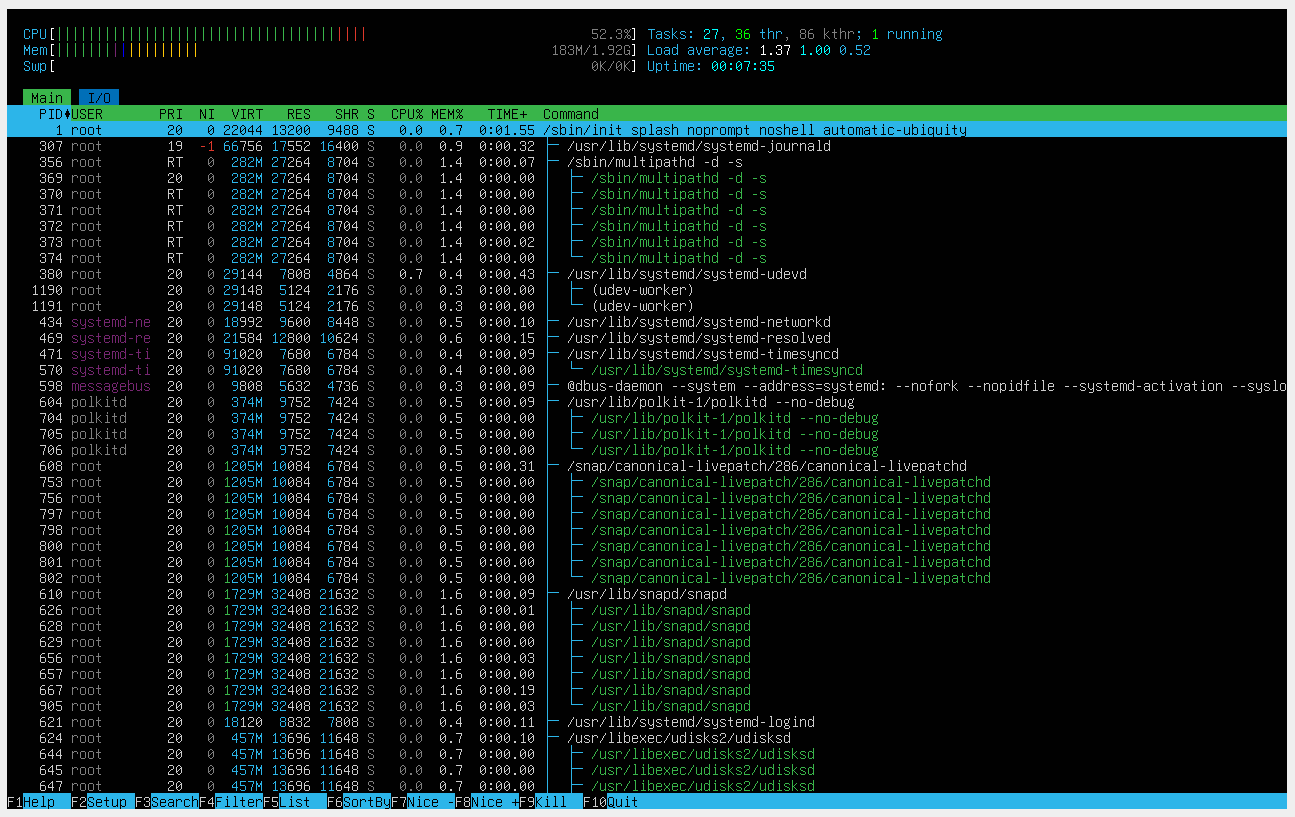
\includegraphics[width=\textwidth]{./images/medcpuload.png}
    \caption{\mintinline{python}{htop} output when running \mintinline{shell}{python3 stress_cpu.py --load medium}}
\end{figure}

\begin{figure}[H]
    \centering
    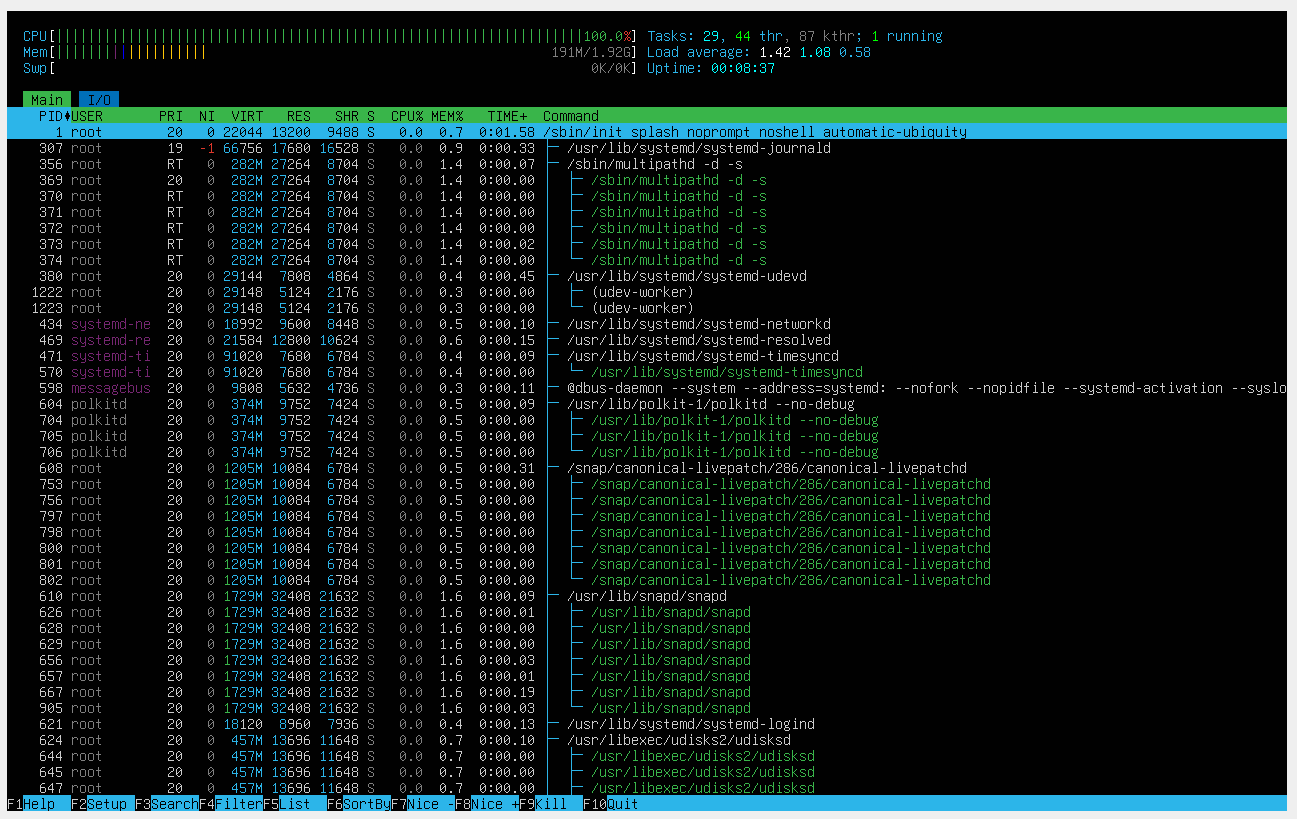
\includegraphics[width=\textwidth]{./images/highcpuload.png}
    \caption{\mintinline{python}{htop} output when running \mintinline{shell}{python3 stress_cpu.py --load high}}
\end{figure}

\begin{code}
\inputminted[linenos, breaklines, frame=single]{python}{../code/stressers/stress_memory.py}
\caption{\texttt{stress\_memory.py}}
\end{code}

\begin{figure}[H]
    \centering
    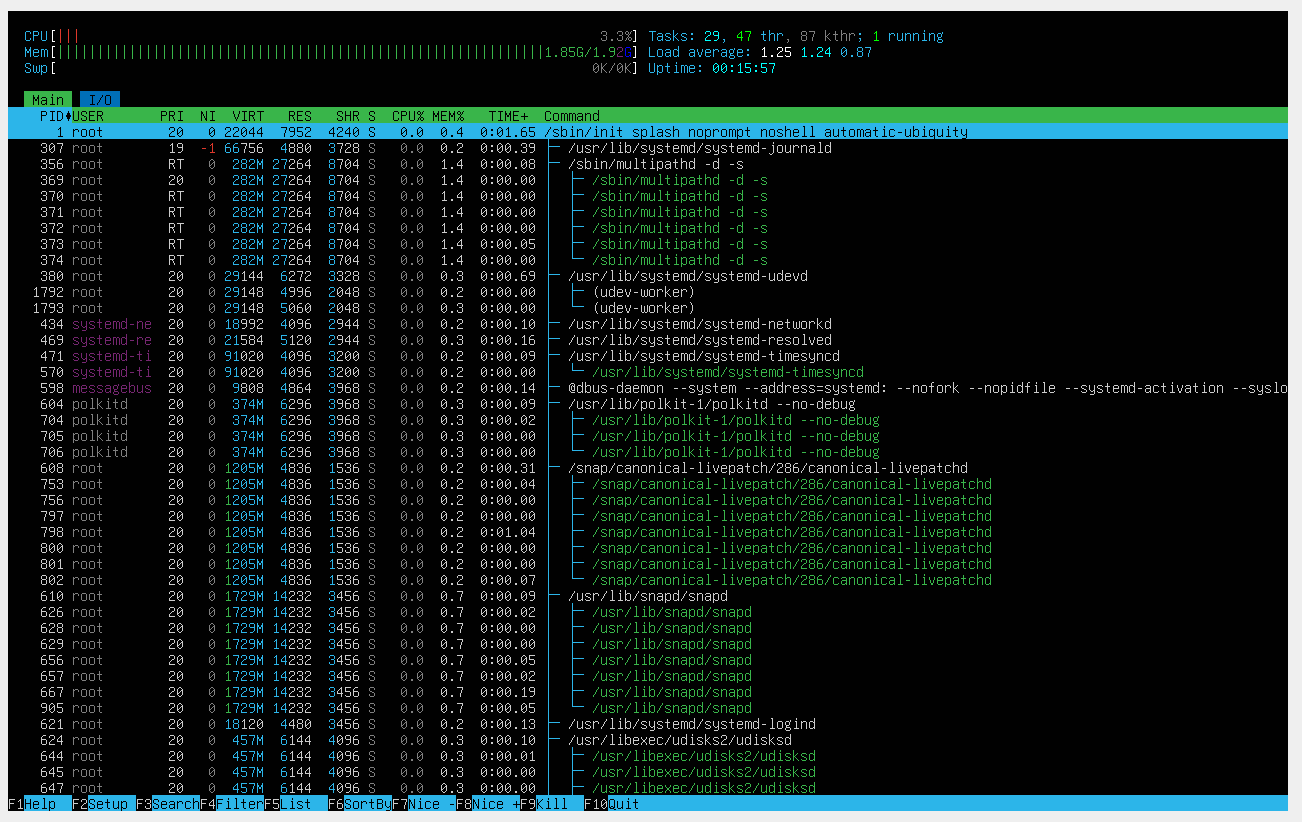
\includegraphics[width=\textwidth]{./images/memstress.png}
    \caption{\mintinline{python}{htop} output when running \mintinline{shell}{python3 stress_memory.py --usage 0.85}}
\end{figure}

\printbibliography
\end{document}
